% *************************************************************************
\chapter[Working title: Calculations]
{Working title: Calculations\label{ch1}}
\chapauth{Martin R. Hediger$^{a}$, Harm Otten$^{b}$
\chapaff{$^{a}$Z\"urich\\
$^{b}$K{\o}benhavn\\
m---@---.ch\\
harm.otten@maxlab.lu.se}}
% *************************************************************************


% *************************************************************************
% *************************************************************************
\section{Motivation}\label{sec:mot}
Let us imagine two companies A and B.
Both companies use very similar technical equipment to carry out the biotechnological process $\ce{a}$ $\xrightarrow{Enzyme}$ $\ce{b}$ using two individual versions of the indicated catalyst.
Company A uses an enzyme with a rate constant $k_\text{A} = 1000s^{-1}$ while company B uses an enzyme with $k_\text{B} = 2000s^{-1}$.
Letting all other things be equal, the process of company B will therefore only require half the time to produce one Mole of product compared to the time required for company A.
Company B therefore can save energy required to keep the reaction volume at a certain temperature.
The need for efficient catalysts arises from such an outline and the commercial implications of these considerations are immediate.\footnote{We use the terms \textit{enzme} and \textit{bio-}/\textit{catalyst} interchangeably.}\\
Increasing the performance of enzymes however is still far from trivial and forms a growing body of research.
What is clear though is that the development of such catalysts is costly, in terms of manpower, material and energy -- if carried out in the laboratory.
A number of companies have in fact formed around this demand: Novozymes (DK), Genzyme (US) or DSM (NL) to name but a few\cite{meyer2013use, kirk2002industrial, beilen2002enzyme, schmid2002use}.\\
Laboratory costs can however be saved to a large part if the development is carried out \textit{in silico}.
The proof that computational results are as reliable as experimental results has been provided not too long ago\cite{claeyssens2006high}.
The foundation for successful application of computational enzyme engineering has thus been laid out.
It is therefore natural to ask: Why hasn't this become more important yet?
Why are there not more job openings at pharmaceutical and biotechnology companies looking for computational enzyme engineers?
The field, after all, did receive the Nobel price in Chemistry 2013.\\
By giving an overview and some details in this article, we hope to also, at least in part, answer these questions.
% *************************************************************************


% *************************************************************************
% *************************************************************************
\section{Introduction}\label{sec:intro}
We provide an introduction into the topic of enzyme catalysis modeling for interested people from inside and outside of the field.\\
We outline the latest achievements, methods in use and outline required developments to establish computational enzyme engineering not only in the literature, but also in (commercial) practice.\\
Modeling involving enzymes happens in different forms.
In one form, the enzyme is a constant parameter and the variable is the inhibitor.
These tasks are usually addressed by docking approaches and studies involving millions of substrates have been published\cite{zhou2010high}.
In another form, the substrate is constant but the enzyme can vary.
The approaches to this task, as it appears, are much less established.
The reasons are manifold, primarily it appears that modeling of an enzyme is less straightforward than a small inhibiting molecule.
Again, why is that?

As is known in the community, enzymes behave highly non-predictable.
The best reasoning about a mutation (except for elimination of the catalytic residues) will not even allow to decide \textit{qualitatively} if the mutated enzyme will be more or less active.
Shifts in pH optima might be predicted more readily\cite{ludwiczek2013strategies}.
It is proposed therefore that in cases where no \textit{a priori} knowledge about how an enzyme should be engineered is available, the only reasonable strategy is to carry out systematic screening studies.
For these to be feasible, either the computer power needs to be very large or the method has to be fast, there is an inherent trade off in this situation.
Once initial lead structures are identified, higher level methods can be used to narrow down on most promising candidates.

This review is written for a more general audience.
For specialized details, the reader is referred to the primary literature.
The intention is to provide an accessible introduction into the field of quantum chemical modeling of enzymatic reactions, highlight advantages of using quantum chemistry and also point out points where special care needs to be taken.
% *************************************************************************


% *************************************************************************
% *************************************************************************
\section{Methods}\label{sec:methods}
A variety of methods has been established for the use to model enzyme catalysis.
Depending on the properties of interest, the system is treated differently.
Molecular mechanics methods allow to study the structural behavior of the enzyme over a significant time period and provide details about rearrangement of loop motives.
The description of chemical reactivity however requires the description of the electronic structure of the system (molecular mechanics models do not allow the description of bond formation and braking processes).
In this regime, again a number of specialized methods have become available.

\subsection{Idea collection}
Practical applicability of QM based enzyme screening has a couple of problems:
\begin{itemize}
\item The structures of the enzyme in the relevant state of the reaction need to be available, ie. an enzyme-substrate complex (ES) and a transition state (TS) analog (usually an inhibited species)
\item If the mechanism is not established, the reaction can usually follow various pathways -- these would need to be checked in order to find a best guess at the rate determining step
\item Identification of the transition state is difficult and depends intimatly on the structure, optimizing two structures differing by 0.1 \AA in a particular bond length can result in identification or not identification of the TS
\item \textit{Every method has it's chemistry}. The results of one QM chemistry need to be verified, usually high-level standard reference methods are computationally too demanding to be applicable to a large system
\item Modeling software is available, PyMOL, Schr\"odinger, Chem?? (Walter Thiel, commercially) but everything is still very much custom work (especially the data analysis, programs output format is like from last century), this is probably the major reason preventing the use of QM as standard method in industry. Compare docking and MD methods have software which is designed towards user friendlyness and has become established in industry
\item GTKDynamo is an exceptionally good example for what it should look like, unfortunately only small community
\item Many papers claim that ``\textit{future developments are directed at further automating the presented approach}''.
Obviously these remarks are directed at making the method industrially applicable by avoiding the requirement to carry out complicated setup and configuration steps\cite{rathore2013advances}.
In reality, such future developments, to the great unfortune of the whole field, are rarely realized -- speculation on the reasons is beyond the scope of this article.
Nevertheless, almost no publication fails to mention the potential applications in drug design.
\item Computational considerations are only rarely taken into account but greatly help at putting the whole approach into perspective: ``\textit{We do not think that this approach is that relevant for high-throughput screening for several reasons.
First, the amount of calculations required for a single compound is not scalable to thousands or millions of ligands, and second, because the degree of detail provided by the methodology is probably not needed during the screening phase.
Instead, we en- visage a successful application in the lead optimization phase on possible tens of lead compounds to completely reconstruct and understand their binding pathways before moving forward in the pipeline.
The method, although computationally expensive, is certainly feasible if performed on just a few ligands as indicated.
Here, we have made use of our volunteer GPU project GPUGRID.net (7) based on ACEMD (6).
Extrapolating from the current study, it would be possible to reconstruct the binding pathways of 5 to 10 ligands per week in-house on a moderately sized GPU cluster of 32–64 GPUs.}''\cite{buch2011complete}
\end{itemize}

\subsection{Calculation methods}
Different methods used should be briefly described to make it easier for the reader of the literature to understand what is going on
\begin{itemize}
\item AM1/RM1/PM3/PM6/PM7/MOZYME
\item DFT/B3LYP/Dispersion corrections/M06/...
\item Modeling procedures: Define constraints- how does it affect the calculation (examples in literature?)
\end{itemize}
% *************************************************************************


% *************************************************************************
% *************************************************************************
\section{Applications}\label{sec:apps}

\subsection{Method Hediger}
We have presented recently a number of studies where new functionality has been introduced into an enzyme active site using quantum chemical methods\cite{10.1371/journal.pone.0049849,hediger2013silico,hediger2013computational}.\\
Rational arguments alone are not sufficient to design new reactivity in an active site.
Put simply, enzymes do not behave in the way the engineer hopes for.
Much rather, the only meaningful strategy proves to be to screen a large number of variant candidates for apparent activity of the desired sort.
In a second step, identified lead candidates are subjected to higher level computational methods and wet-lab experiments which then allow to further establish or dismiss the nature of the candidate.
Based on the vast mutational space available, initial \textit{in silico} screening has to be efficient.
Hediger \textit{et al.} therefore chose to use semi-empirical methods for the description of the electronic structure of the enzyme-substrate complex.
In their approach, the activities of different variants of an enzyme are ordered by comparing the activation energy required for the rate determining step of the overall reaction -- low activation energies correspond to high anticipated activity of the variant.

In the following, the basic procedure consists of preparing structures for the enzyme substrate complex (``ES'') and the first intermediate (CALB: ``TI''/Tetrahedral intermediate, BCX: ``GE''/Glycosyl enzyme) and calculating the reaction barrier between these two structures, respectively.
The reaction barrier is calculated by preparing intermediate structures of the model along the reaction coordinate ES$\rightarrow$TI or ES$\rightarrow$GE.
The quality of the results of the study are strongly dependent on how careful the modeling of these structures is carried out, a major reason for meaningless results is significant structural rearrangement during the geometry optimization.

\subsubsection{{\textit{Candida antarctica} Lipase B Engineering}}
Introducing amidase functionality into the lipase of \textit{Candida antarctica} (CALB).

CALB is used as a versatile catalyst in a variety of applications among which enzymatic kinetic resolution of enantiomeric mixtures is of high pharmaceutical importance\cite{gotor2006candida}.
While CALB is also known for its reactive promiscuity\cite{CBIC:CBIC200800318}, if the catalyst can be engineered such as to increase its performance for certain of these applications, possible bottle-necks in production could be widened.\\
About the cutoff: this is only relevant in studies where experimental data for many mutants is available.
Then it can be used to assess the lower barrier for the accuracy.
Given all approximations, x out of y mutants are correctly predicted.
So any method improving on the approximations should provide at least at many correct hits.\\
About the cutoff: this is only relevant in studies where experimental data for many mutants is available.
Then it can be used to assess the lower barrier for the accuracy.
Given all approximations, x out of y mutants are correctly predicted.
So any method improving on the approximations should provide at least at many correct hits.

\subsubsection{\textit{Bacillus circulans} xylanase engineering}
As a proof of concept and to show general applicability of the approach outlined for CALB, the xylanase of \textit{Bacillus circulans} is engineered to be catalytically active towards an artifical substrate.
Importantly, we note that the same method as developed for computational screening of CALB activity could be directly transfered to the study of BCX activity.
The requirements are that a structure representing a bound intermediate along the reaction pathway is available.
Ideally, the mechanism for the rate determining step is established in the literature, however this is not a critical requirement.
In this study, the mechanism was taken from the literature as reported previously\cite{joshi2000hydrogen,joshi2001dissecting}.
If the mechanism is not established, the method can just as well be used to outline competing mechanisms.\\
%Outline scientific/systematic approach taken in paper.
%Does the result depend on the method?
%Does the result depend on the modeling sequence?
%Does the result depend on the size of the model?
%Systematic preparation of all possible mutants, i.e. the conclusions do not depend on the selection of the mutants taken in paper.
%Does the result depend on the method?
%Does the result depend on the modeling sequence?
%Does the result depend on the size of the model?
%Systematic preparation of all possible mutants, i.e. the conclusions do not depend on the selection of the mutants.
The paper follows the following reasoning in order to establish independence of results on modeling procedure and internal consistency within the framework of approximations (both from the quantum chemical model as well as the limited including of physical effects).
In a first step, the wild-type (WT) reference reaction barrier height is established.
This is a crucial step because all subsequent conclusions about mutants are depending on how good the WT reaction barrier is estimated.
As noted above, only the rate determining step is modeled, Fig. \ref{fig:bcx_mechanism}.
\begin{figure}[htbp] 
\centering
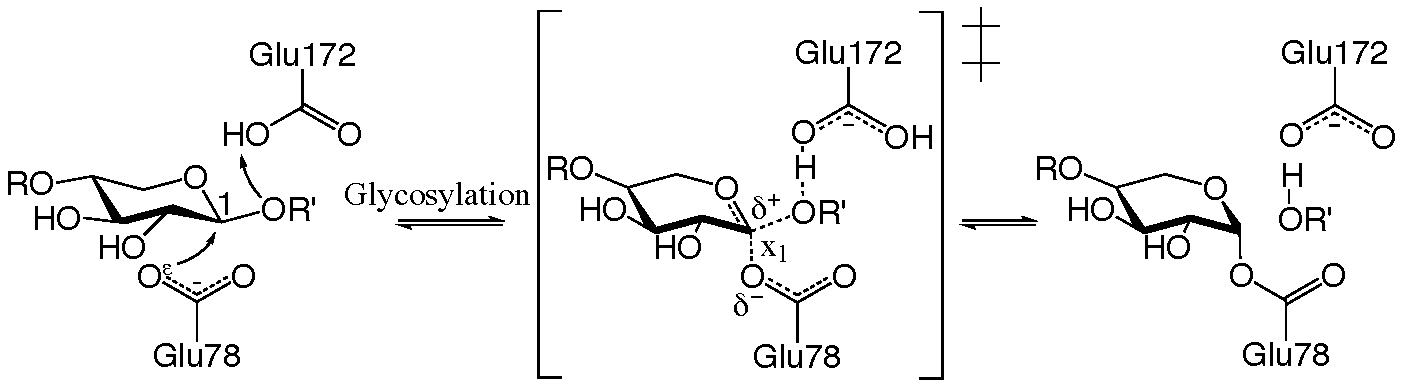
\includegraphics[width=1.0\linewidth]{mechanism.pdf}
\caption{
Conventional glycosylation step. $x_1$: constrained reaction coordinate; $R$: xylose; 
$R'$: \textit{ortho}-nitrophenol (ONP).
%For discussion of proton transfer from E172 to substrate, see text.
C$_1$ indicating nucleophilic carbon of first xylose unit.
}
\label{fig:bcx_mechanism}
\end{figure}
As outlined in the methods section, the reaction barrier is mapped out by fixing the reaction coordinate at a fixed interval while optimizing the rest of the protein structure.
Since the reaction consists of two concerted events (nucleophilic attack by E78 and proton transfer from E172 to ONP), in principle a two-dimensional potential energy surface could be mapped out to determine the reaction barrier.
However, since proton transfer is associated with a rearrangement of the electronic structure, this reaction coordinate is not constrained and the proton is free to transfer or remain on E172.
In simple terms, forcing the quantum chemistry to do something it would not if unconstrained would result in an increased reaction barrier and therefore it is advisable to keep the number of constraints as low as possible.\\
\textbf{Molecular modeling steps}\\
While considering only a subset of the residues in the active site for the model, as done for CALB, introduces some ambiguity, in this study the full structure of BCX was included in the model.
The modeling approach should consider the structures available.
In this case, a PDB structure using a covalent inhibitor is available (1BVV) and this is a good starting point for the modeling procedure because it gives a very clear indication of how the substrate is located in the active site.
There is also an apoenzyme of BCX available, however placing a substrate into an empty active site requires considerable rearrangement of active site residues.
Furthermore, ambiguity in how the substrate should be placed in the active site can be reduced using the structure including the inhibitor, which is important in order to increase reproducibility of the research.
As shown in Fig. 2 of the paper, two possible modeling pathways were worked out.
In the first one, the ES complex is prepared from the GE structure \textit{before} the GE structure is optimized, in the second (``Interpolation 2''), first the GE structure is optimized and only then is the ES structure prepared.
The main advantage of the second approach is that a significant amount of computer time can be saved because a large part of the enzyme is already optimized when the ES structure is prepared.two possible modeling pathways were worked out.
In the first one, the ES complex is prepared from the GE structure \textit{before} the GE structure is optimized, in the second (``Interpolation 2''), first the GE structure is optimized and only then is the ES structure prepared.
The main advantage of the second approach is that a significant amount of computer time can be saved because a large part of the enzyme is already optimized when the ES structure is prepared.


\subsection{Interesting QM/MM applications}
\textbf{The cocaine hydrolase guys}\\
Make a cocaine hydrolase better\cite{gao2006computational}.

\subsection{Requirements for advancement of methods}
Experimental catalytic data ($k_\text{cat}$) of many mutants to validate against.
% *************************************************************************


% *************************************************************************
% *************************************************************************
\section{Conclusions}\label{sec:conclusions}

\subsection{Advantages/Disadvantages of using quantum chemistry for modeling enzymatic reactions}
\begin{itemize}
\item Bond formation/breaking can be modeled
\item Large systems might require constraints to reach convergence
\item Calculation times depend strongly on model chemistry used
\item Not yet as established and convenient to use like e.g. docking software
\end{itemize}
